\beginsong{Wir sind des Geyers}[wuw={nach Gedichten von Heinrich v. Reder, Musik: Nerother Wandervogel, 1919}, pfii={25}, bo={400}]

\markboth{\songtitle}{\songtitle}

\beginverse
\endverse

\centering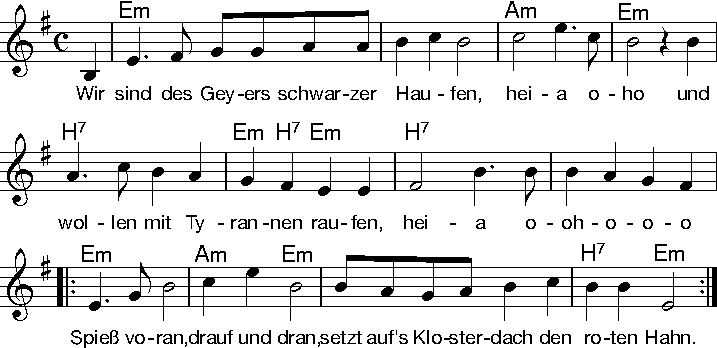
\includegraphics[width=1\textwidth]{Noten/Lied099.pdf}

\beginverse

Als \[Em]Adam grub und Eva spann, \[Am]Kyrie\[Em]leis,
wo \[H7]war denn da der \[Em]E\[H7]del\[Em]mann, \[H7]Kyrieleis.

\endverse

\beginchorus
\lrep \[Em]Spieß voran, \[Am]drauf und \[Em]dran, setzt auf's Klosterdach den \[H7]roten \[Em]Hahn. \rrep
\endchorus

\beginverse


Jetzt ^gilt es Schloss, Abtei und Stift, ^hei-a o^ho
uns ^gilt nichts als die ^heil'^ge ^Schrift, ^hei-a oho

\endverse

\renewcommand{\everychorus}{\textnote{\bf Refrain (wdh.)}}
\beginchorus
\endchorus
\beginverse
 
Des ^Edelmannes Töchterlein, ^Kyrie^leis,
wir ^schicken's in die ^Höll' ^hi^nein, ^Kyrieleis.

\endverse

\beginchorus
\endchorus
\beginverse


Uns ^führt der Florian Geyer an, ^trotz Acht und ^Bann,
den ^Bundschuh führt er ^in ^der ^Fahn, hat ^Helm und Harnisch an.
\endverse

\beginchorus
\endchorus
\beginverse



Bei ^Weinsberg setzt es Brand und Stank, ^hei-a o^ho,
gar ^mancher über die ^Klin^ge ^sprang, ^hei-a oho.

\endverse

\beginchorus
\endchorus
\beginverse


Ge^schlagen ziehen wir nach Haus, ^hei-a o^ho,
unsre ^Enkel fechten's ^bes^ser ^aus, ^hei-a oho.

\endverse

\beginchorus
\endchorus

\endsong

\beginscripture{}
Wir sind des Geyers ist ein nach dem Ersten Weltkrieg entstandenes politisches Kampflied, das die Taten des Florian Geyer und seines Schwarzen Haufens, einer Odenwälder Bauernarmee, während der Bauernkriege des 16. Jahrhunderts glorifiziert.
Der Text des Liedes entstand um 1920 in Kreisen der Bündischen Jugend. Das Lied wurde vom Nationalsozialismus im Kampf gegen die katholische Kirche eingesetzt. Außerdem gehörte es zum offiziellen Liedgut der SS. Während des Zweiten Weltkrieges gab es eine Kavallerie-Division der Waffen-SS namens Florian Geyer. Sehr oft findet man in Liederbüchern nur Teile des Liedes und diese in abgeschwächter Form. Die ursprüngliche Version hat 13 Strophen.
\endscripture

\begin{intersong}

\end{intersong}